\documentclass[tikz,border=4pt]{standalone}
% Shared style for MultiMM figures (white background, logo palette)
\usepackage{tikz,pgfplots,amsmath}
\pgfplotsset{compat=1.16}
\usetikzlibrary{arrows.meta,calc,decorations.pathreplacing,positioning,backgrounds}
\definecolor{indigo}{HTML}{3B37A0}
\definecolor{violet}{HTML}{6A3AA8}
\definecolor{crimson}{HTML}{B5406C}
\definecolor{gold}{HTML}{E9A62C}
\definecolor{golddark}{HTML}{B9791A}
\definecolor{grey}{HTML}{8A8AA0}
\definecolor{lightgrey}{HTML}{E4E4EE}
\tikzset{
  bead/.style={circle,draw=#1!80!black,fill=#1!35,line width=0.5pt,minimum size=9pt,inner sep=0pt},
  bead/.default=indigo,
  lab/.style={font=\small},
}
\pgfplotsset{
  every axis/.append style={
    width=9.5cm,height=6.3cm,axis lines=left,line width=0.5pt,
    grid=major,grid style={draw=lightgrey,line width=0.3pt},
    tick label style={font=\small},label style={font=\normalsize},
    legend style={font=\footnotesize,draw=none,fill=white,fill opacity=0.8,text opacity=1},
    legend cell align=left,
  },
  every axis plot/.append style={line width=1.2pt,smooth},
}

\begin{document}
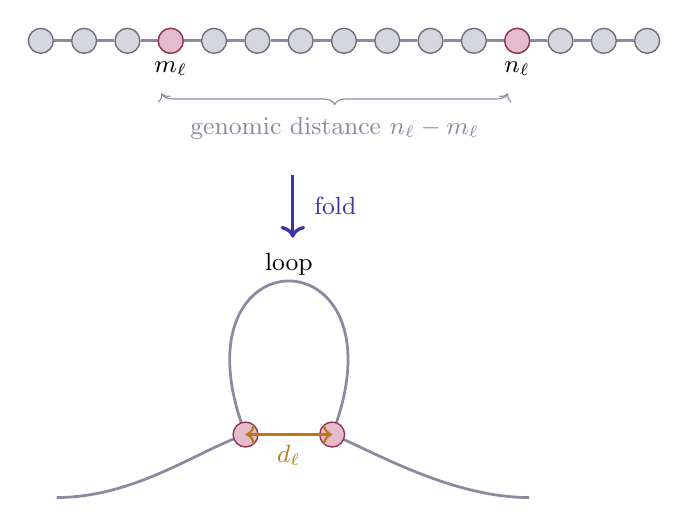
\begin{tikzpicture}
% linear chain with two anchors
\foreach \i in {0,...,14}{\node[bead=grey] (c\i) at (\i*0.55,0) {};}
\foreach \i in {0,...,13}{\pgfmathtruncatemacro{\j}{\i+1}\draw[grey,line width=1pt] (c\i)--(c\j);}
\node[bead=crimson] at (c3) {}; \node[bead=crimson] at (c11) {};
\node[lab,below=4pt] at (c3) {$m_\ell$}; \node[lab,below=4pt] at (c11) {$n_\ell$};
\draw[<->,decorate,decoration={brace,mirror,amplitude=4pt},grey] (c3.south west)++(0,-0.55) -- ++(4.4,0) node[midway,below=5pt,lab] {genomic distance $n_\ell-m_\ell$};
\draw[->,line width=1.2pt,indigo] (3.2,-1.7)--(3.2,-2.5);
\node[lab,indigo,anchor=west] at (3.35,-2.1) {fold};
% folded loop
\begin{scope}[shift={(0,-6.0)}]
\foreach \i/\a in {0/200,1/230,2/260}{}
\coordinate (m) at (2.6,1.0); \coordinate (n) at (3.7,1.0);
\draw[grey,line width=1pt] (0.2,0.2) .. controls (1.2,0.2) and (2.0,0.8) .. (m);
\draw[grey,line width=1pt] (m) .. controls (1.6,3.6) and (4.7,3.6) .. (n);
\draw[grey,line width=1pt] (n) .. controls (4.2,0.8) and (5.2,0.2) .. (6.2,0.2);
\node[bead=crimson] at (m) {}; \node[bead=crimson] at (n) {};
\draw[<->,golddark,line width=0.8pt] (m)--(n) node[midway,below,lab] {$d_\ell$};
\node[lab,above] at (3.15,2.9) {loop};
\end{scope}
\end{tikzpicture}
\end{document}
